\subsection{Pseudosphere}
\label{sec:pseudosphere}

The sphere is a surface with constant positive curvature.
Are there surfaces with constant negative curvature?
The answer is yes, one such surface is the pseudosphere
which we introduce here. We will then use the Gauss-Bonnet
theorem to determine the Euler characteristic of the pseudosphere as
shown in \cite{pseudo-app}.


The tractrix is the curve whose tangent meet the $x$-axis a unit distance
from the point of tangency \cite{thurston}. See \figref{tractrix} for an illustration.
Intuitively, imagine a bike with unit distance between where the tires meet the ground.
Place the back wheel on the positive $y$-axis and front wheel on the origin pointed
toward the positive $x$-axis. We then push the bike forward while keeping the front
wheel on the $x$-axis. Then do the same in the negative $x$ direction.
The tractrix is the curve traces by the back tire. 


\begin{figure}[htb]
    \captionsetup[subfigure]{justification=centering}
    \centering
    \begin{subfigure}[b]{0.4\textwidth}
        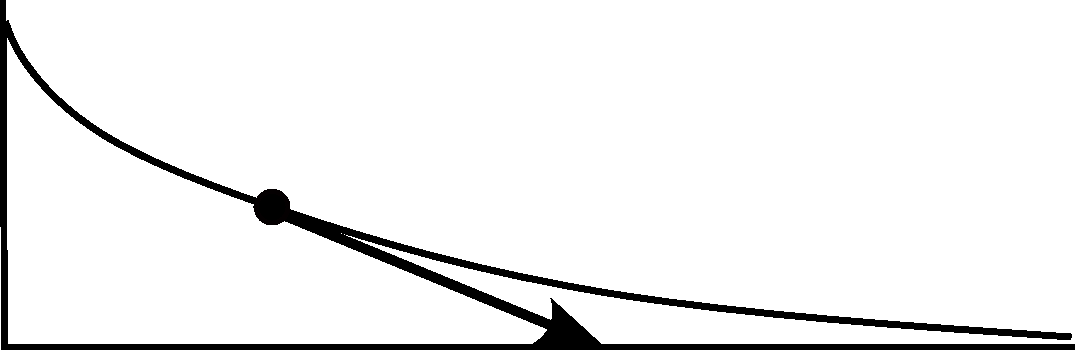
\includegraphics[width=\textwidth]{pseudosphere/tractrix}
       \subcaption{}\label{fig:tractrix}
    \end{subfigure}
        \hspace{1cm}
        \begin{subfigure}[b]{0.4\textwidth}
        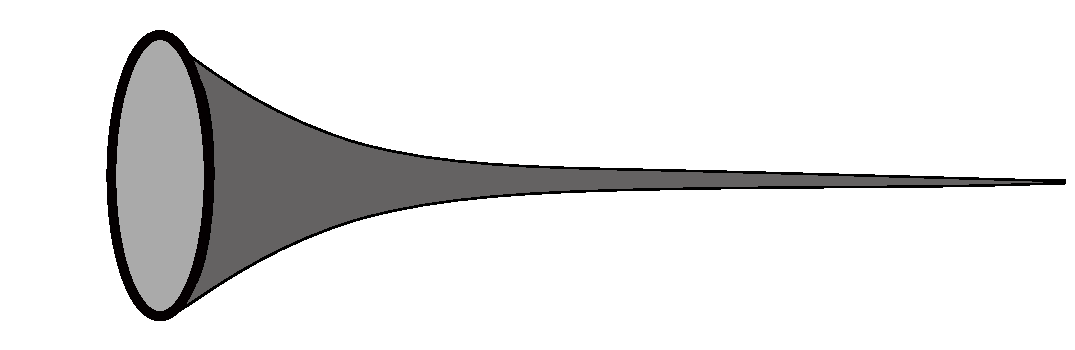
\includegraphics[width=\textwidth]{pseudosphere/pseudosphere}
        \subcaption{}\label{fig:pseudosphere}
        \end{subfigure}
    \caption{(\subref{fig:tractrix}) The length of the tangent vector from a point to the $x$-axis is one.
        (\subref{fig:pseudosphere}) The truncated pseudosphere.
    }
    \label{fig:tractrix-pseudosphere}
\end{figure}



The pseudosphere is the surface formed by rotating the tractrix around the $x$-axis.
An example is shown in \figref{pseudosphere}.
One can show that the curvature of a surface of revolution formed by rotating a curve
$(x(t),y(t)),$ where $t$ is the arc length, about the $x$-axis is given by

$$K=-\frac{1}{y}\frac{d^2t}{dt^2}$$
and conclude that the curvature is negative one.
Using the well know formula for the surface area of a surface of revolution
we see that the area of the pseudosphere is $4\pi$.

Suppose we wish to compute the Euler characteristic of half of the pseudosphere,
the Gaussian curvature is $-1$ and the area is $2\pi$, we need to compute
the geodesic curvature of the boundary. 

The boundary occurs where $x=0$, we should also consider what happens as $x$ approaches
infinity.  When $x=0$ the boundary is a unit circle 
$$c(t)=(\cos(t),\sin(t),0),$$ using the \eqnref{geodesic}, we have
$$k_g=\langle c''(t),(N\times c'(t))=1.$$
Plugging into the Gauss-Bonnet theorem we see that
the Euler characteristic of the top half of the pseudosphere is zero!



